\chapter{ALoVaS Examples and a Case Study}\label{sec:Examples}

In this chapter we present simulation studies to illustrate properties of our methods. The two illustrated properties are handling multi-modality and handling highly non-balanced categorical response variable class probabilities. Following these simulation studies we present a case study using the internet ads dataset from the UC-Irvine machine learning database \cite{Frank:2010uq}. 

We first present simulated examples where we study the efficacy of our proposed method. We use the regularization priors we describe in Chapter \ref{sec:Introduction}. Concluding Section \ref{sec:real_data}, we give an example classifying webpages according to whether those webpages contain ads or not. Finally, in Section \ref{sec:Conclusion}, we summarize our findings and discuss the limitations, extensions, and possible variations of the ALoVaS model.     

	\section{Simulated Examples}
	In this section we present two collections of simulations. The first collection aims to study the effects of having multiple best trees in the generative model. The second collection aims to study the effects of class imbalance when dealing with a categorical response. 
	
%\subsubsection{Correlated Covariate Simulations}
%		
%		\begin{figure}[H]
%  \centering
%  \includegraphics[width=4in]{figures/scaled_shifted_beta_plots_bw.pdf}
%  \caption{Plots of the scaled-beta densities for the parameter settings we use to simulate correlation parameters. }
%  \label{fig:scaled_shifted_beta}
%\end{figure}
%
%We simulate data according to the linear regression model given by Equation \ref{def:linear_model}. The $X$ matrix contains row vectors of covariates denoted $\vec{x}_i^T$. The covariates are draws from a correlated multivariate normal density with the correlation matrix given by $4\nu I + \rho J$, where $I$ and $J$ are conformable identity and and all 1 matrices respectively. The parameter $\nu$ is sampled from an inverse gamma distribution with shape and scale parameters of $1/2$ and $1$. The parameter $\rho$ is sampled from one of the beta distributions given in Figure \ref{fig:scaled_shifted_beta} depending on which correlation scenario is given. Moreover, we simulate the random coefficients, $\vec{\mu}$, according to a continuous uniform distribution on the support $[-20,20]$. Thus, our simulations have scenarios of highly and weakly correlated covariates, as well as both positive and negative coefficients.
%
%%%% table of simulation results for correlated covariates simulations. 
%
%\begin{table}[H]
%\begin{center}
%\begin{tabular}{cc|c|c|c|c|c|c|}
%\cline{3-8}
%& & \multicolumn{6}{|c|}{Correlation Scenarios }\\  \cline{3-5}
%& & All High & All Mid & All Low  \\\cline{1-5}
%\multicolumn{1}{ |c| }{\multirow{3}{*}{50\% Sparsity} }  &
%\multicolumn{1}{ |c| }{SSVS} & 719679.05 &605340.89  &259739.80    \\  \cline{2-5}
%\multicolumn{1}{ |c| }{}&LASSO&321976.86  & 289537.96& 185282.31    \\ \cline{2-5}
%\multicolumn{1}{ |c| }{}&HORSESHOE  & 653732.97 &153722.46  &  445669.36 \\ \cline{1-5} 
%\multicolumn{1}{ |c| }{\multirow{3}{*}{60\% Sparsity} }  &
%\multicolumn{1}{ |c| }{SSVS} &591305.83  &507564.78  & 140295.82   \\  \cline{2-5}
%\multicolumn{1}{ |c| }{}&LASSO& 681873.23 &803175.40  &112567.28    \\ \cline{2-5}
%\multicolumn{1}{ |c| }{}&HORSESHOE  & 317808.78 & 205273.51 &199787.11   \\ \cline{1-5} 
%\multicolumn{1}{ |c| }{\multirow{3}{*}{70\% Sparsity} }  &
%\multicolumn{1}{ |c| }{SSVS} &42107.02  &36544.59  & 72987.87   \\  \cline{2-5}
%\multicolumn{1}{ |c| }{}&LASSO& 54788.10 & 26672.33 &  57799.72    \\ \cline{2-5}
%\multicolumn{1}{ |c| }{}&HORSESHOE  &62239.98& 33495.43 & 65066.95  \\ \cline{1-5} 
%\multicolumn{1}{ |c| }{\multirow{3}{*}{80\% Sparsity} }  &
%\multicolumn{1}{ |c| }{SSVS} &25452.16&28720.73 &4039.34 \\  \cline{2-5}
%\multicolumn{1}{ |c| }{}&LASSO&21379.87  &21292.66  &  3174.12     \\ \cline{2-5}
%\multicolumn{1}{ |c| }{}&HORSESHOE  & 34541.69 & 44203.84 & 2266.33  \\ \cline{1-5} 
%\multicolumn{1}{ |c| }{\multirow{3}{*}{90\% Sparsity} }  &
%\multicolumn{1}{ |c| }{SSVS} &18639.01 & 2299.55 &1302.07    \\  \cline{2-5}
%\multicolumn{1}{ |c| }{}&LASSO&20570.07  & 2877.12 &1467.92\\ \cline{2-5}
%\multicolumn{1}{ |c| }{}&HORSESHOE  & 27485.12 &1278.87  & 3230.96  \\ \cline{1-5} 
%\multicolumn{1}{ |c| }{\multirow{3}{*}{95\% Sparsity} }  &
%\multicolumn{1}{ |c| }{SSVS} &89319.59 &1309.86 &4894.39      \\  \cline{2-5}
%\multicolumn{1}{ |c| }{}&LASSO& 79849.77 & 1507.78 & 1124.96      \\ \cline{2-5}
%\multicolumn{1}{ |c| }{}&HORSESHOE  &21061.88 & 4186.80 & 1260.12  \\ \cline{1-5} 
%\multicolumn{1}{ |c| }{\multirow{3}{*}{99\% Sparsity} }  &
%\multicolumn{1}{ |c| }{SSVS} &12031.52  &2383.80  &1233.37    \\  \cline{2-5}
%\multicolumn{1}{ |c| }{}&LASSO&19271.86  &1287.68 & 1231.78     \\ \cline{2-5}
%\multicolumn{1}{ |c| }{}&HORSESHOE  &16897.56  &1726.18  & 3282.69 \\ \cline{1-5} 
%\end{tabular}
%\caption{Correlated simulation study results, each entry represents the MSE for that scenario and model. The MSE is calculated as $\sum_{i}(\hat{y}_{i}-y_i)^{2}/10000$, where $i$ runs from draw $1,000$ to $11,000$. Thus our burn-in is $1,000$.}
%\label{tab:corr_study_results}
%\end{center}
%\end{table}
%%%% end of table of simulation results for the correlated covariates simulations
%
%What is apparent from Table \ref{tab:corr_study_results} is that there is no clearly better flavor of ALoVaS. The choice of which method works best is likely to depend on the correlations of the covariates and the degree of sparsity present in the underlying data generating process. Moreover, We notice an increase in the mean squared prediction error as the sparsity decreases, in particular we notice a large increase as we move from a 90\% sparse data generating process to one that is less sparse. This corresponds with findings from Monte Carlo simulations the authors have conducted on the linear model equivalents of the three ALoVaS models. The finding that the best choice of method depends on unknown and difficult to estimate parameters is troubling from a practical standpoint. While it may be taken as a given that in genomics problems the sparsity of the underlying model is 99+\%, in many other application areas like insurance, econometric, and environmental statistics to name a few, the degree of sparsity is not so clear and may vary from less than 10\% to over 99\% depending on the data and the phenomenon being modeled.  

\subsection{Multimodal Simulation Study}
In this collection of simulations we study is a class of simulations where more than one model explains the data equally well. We simulate data according to the model described in Wu, Tjelmland, and West \cite{wu2007bayesian}, which exhibits multi-modality, also called the Rashomon effect by Breiman \cite{breiman2001statistical}. To simulate effectively from the data generating process, we need to be able to sample the two models in the same chain. 

For this simulated example we take $x_{i1} \sim \text{Unif}(.1,.4)$, for $i=1,\dots ,200$, and $x_{i1} \sim \text{Unif}(.6,.9)$, for $i=201,\dots,300$. Similarly, $x_{i2} \sim \text{Unif}(.1,.4)$, for $i=1,\dots ,100$, $x_{i2} \sim \text{Unif}(.6,.9)$, for $i=101, \dots,200$ , and $x_{i2} \sim \text{Unif}(.1,.9)$, for $i=201, \dots,300$. Finally, $x_{i3} \sim \text{Unif}(.6,.9)$ for $i =1, \dots 200$, and $x_{i3} \sim \text{Unif}(.1,.4)$, for $i=201, \dots,300$. Then, given these values, 

\[
 y_i =
  \begin{cases} 
      \hfill 1+N(0,0.25)    \hfill & \text{ if $x_{1i} \leq 0.5$ and $x_{2i} \leq 0.5$, } \\
      \hfill 3+ N(0,0.25) \hfill & \text{ if $x_{1i} \leq 0.5$ and $x_{2i} > 0.5$, } \\
      \hfill 5+ N(0,0.25) \hfill & \text{if $x_{1i} > 0.5$. }\\
  \end{cases}
\]

We run our algorithm using the regularized methods on the number of splits and then transform all the sampled $\mu_j$ using the \ALT. In this simulation, varying the sparsity is not something easily parametrized. Whereas in the next simulation we can vary the number of active covariates, in this simulation we must fix the number of active covariates to $3$ and vary the total number of covariates to accomplish a varying of the percentage of sparsity. Similarly to the next simulation, we compare the linear model methods: lasso, horseshoe, and SSVS. so for a sparsity of 50\% we simulate $x_1, \dots, x_6$ with the last three covariates being independent draws from standard normals higher sparsity percentages correspond to a larger number of additional standard normal covariates being independently sampled. The various models correspond to the rows within a sparsity level in Table \ref{tab:rashomon_study_results}.  

\begin{table}[H]
\begin{center}
\begin{tabular}{cc|c|c|c|}
  \\ \cline{3-3}
& & MSE  \\\cline{1-3}
\multicolumn{1}{ |c| }{\multirow{3}{*}{sparsity 50\%} } & 
\multicolumn{1}{ |c| }{CGM} & $34.74 \pm 12.27$\%  \\  \cline{2-3}
\multicolumn{1}{ |c| }{}&SSVS &$12.43 \pm 6.21$\%  \\  \cline{2-3}
\multicolumn{1}{ |c| }{}&LASSO& $5.89 \pm 3.48$\%    \\ \cline{2-3}
\multicolumn{1}{ |c| }{}&HORSESHOE &$7.35 \pm 8.21$ \%  \\ \cline{1-3}
\multicolumn{1}{ |c| }{\multirow{3}{*}{sparsity 60\%} } & 
\multicolumn{1}{ |c| }{CGM} &$34.44 \pm 9.62$ \%  \\  \cline{2-3}
\multicolumn{1}{ |c| }{}&SSVS & $9.64 \pm 5.81$\%    \\  \cline{2-3}
\multicolumn{1}{ |c| }{}&LASSO&$6.19 \pm 2.61$\%     \\ \cline{2-3}
\multicolumn{1}{ |c| }{}&HORSESHOE &$9.22 \pm 7.14$\%  \\ \cline{1-3}
\multicolumn{1}{ |c| }{\multirow{3}{*}{sparsity70\%} } & 
\multicolumn{1}{ |c| }{CGM} &$27.13 \pm 11.83$\%  \\  \cline{2-3}
\multicolumn{1}{ |c| }{}&SSVS &$8.41 \pm 5.79$\%    \\  \cline{2-3}
\multicolumn{1}{ |c| }{}&LASSO&$6.64 \pm 2.63$\%    \\ \cline{2-3}
\multicolumn{1}{ |c| }{}&HORSESHOE &$16.05 \pm 7.23$\%   \\ \cline{1-3}
\multicolumn{1}{ |c| }{\multirow{3}{*}{sparsity 80\%} } & 
\multicolumn{1}{ |c| }{CGM} & $27.64 \pm12.91$\%  \\  \cline{2-3}
\multicolumn{1}{ |c| }{}&SSVS &$8.69 \pm 3.43$ \%   \\  \cline{2-3}
\multicolumn{1}{ |c| }{}&LASSO&$6.12 \pm 1.01$\%    \\ \cline{2-3}
\multicolumn{1}{ |c| }{}&HORSESHOE &$7.52 \pm 5.21$\%  \\ \cline{1-3}
\end{tabular}
\caption{Multimodal simulation study results. Each entry represents the mean squared error of the optimal tree from the Markov chain. The numbers after the $\pm$ are the standard errors across the ten optima for the parallel chains. The $^*$ indicates that 3 cannot be divided by a number to get 60\% sparsity exactly. }
\label{tab:rashomon_study_results}
\end{center}
\end{table}

\begin{table}[H]
\begin{center}
\begin{tabular}{cc|c|c|c|}
  \\ \cline{3-3}
& & MSE  \\\cline{1-3}
\multicolumn{1}{ |c| }{\multirow{3}{*}{sparsity 90\%} } & 
\multicolumn{1}{ |c| }{CGM} &$68.06 \pm 13.76$ \%  \\  \cline{2-3}
\multicolumn{1}{ |c| }{}&SSVS &$11.94 \pm 4.68$ \%   \\  \cline{2-3}
\multicolumn{1}{ |c| }{}&LASSO& $8.41\pm 2.09$\%     \\ \cline{2-3}
\multicolumn{1}{ |c| }{}&HORSESHOE & $ 9.63\pm 7.89$\%   \\ \cline{1-3}
\multicolumn{1}{ |c| }{\multirow{3}{*}{sparsity 95\%} } & 
\multicolumn{1}{ |c| }{CGM} &$47.37 \pm 17.89$\%  \\  \cline{2-3}
\multicolumn{1}{ |c| }{}&SSVS & $7.08 \pm 4.37$\%    \\  \cline{2-3}
\multicolumn{1}{ |c| }{}&LASSO& $11.15\pm 3.70$\%     \\ \cline{2-3}
\multicolumn{1}{ |c| }{}&HORSESHOE &$8.98 \pm 3.88$ \%   \\ \cline{1-3}
\multicolumn{1}{ |c| }{\multirow{3}{*}{sparsity 99\%} } & 
\multicolumn{1}{ |c| }{CGM} & $47.51 \pm 18.31$ \%  \\  \cline{2-3}
\multicolumn{1}{ |c| }{}&SSVS & $6.82 \pm 3.17$\%   \\  \cline{2-3}
\multicolumn{1}{ |c| }{}&LASSO&$7.33 \pm 3.21$\%     \\ \cline{2-3}
\multicolumn{1}{ |c| }{}&HORSESHOE &$5.73 \pm  4.01$\%   \\ \cline{1-3}
\end{tabular}
\caption{Second table of multimodal simulation study results. Each entry represents the mean squared error of the optimal tree from the Markov chain. }
\label{tab:rashomon_study_results2}
\end{center}
\end{table}


 \begin{figure}[H]
  \begin{center}
\begin{tikzpicture}
 \node [circle,draw]{$X_1 \leq 0.5$} [level distance=25mm,sibling distance=50mm]
child { node [circle,draw]{$X_2 \leq 0.5$} [level distance=25mm ,sibling distance=25mm]
child {node [circle,draw] {}}
child {node [circle,draw]{}}
}
child {node [circle,draw] {} [level distance=25mm ,sibling distance=25mm]
};
\end{tikzpicture}
\hspace{1cm}
\begin{tikzpicture}
 \node [circle,draw]{$X_3 \leq 0.5$} [level distance=25mm,sibling distance=50mm]
child { node [circle,draw]{} [level distance=25mm ,sibling distance=25mm]
}
child {node [circle,draw] {$X_2 \leq 0.5$} [level distance=25mm ,sibling distance=25mm]
child {node [circle,draw] {}}
child {node [circle,draw]{}}
};
\end{tikzpicture}
\caption{The two optimal trees for the multimodal simulation study. }
\label{fig:best_two_trees}  
\end{center}
\end{figure}
For the results presented in Table \ref{tab:rashomon_study_results} our burn-in is $1,000$. Additionally, we calculate MSEs using the 10,000 observations after burn in. Convergence diagnostics indicated a minimum sample size of 3746, so 10,000 samples is beyond adequate. 
 
Moreover, in Table \ref{tab:rashomon_study_results} a sentiment appears. There is no clear winner across sparsity levels. While the lasso and the horseshoe appear to be competitive at higher sparsity levels, the SSVS method might also be competitive at lower and higher sparsity levels but there is some degree of variability across the sparsity levels. Additionally, while all three models are able to attain one of the two modes, all three models have difficulty moving from one of the two modes in the underlying model to the other mode. This is exactly a result of the sparsity imposed on the fitted model. The two posterior trees in the two modes have different sets of covariates and thus the sparsity patterns will have difficulty switching from one to the other. A similar pattern can be found in sparse linear models. Typically, correlation constraints are imposed on the $(X^TX)$ matrix to ensure consistency of the selected sparsity pattern. 

\subsection{Class Unbalancedness Simulation Study}
We next perform a simulation on unbalanced response class probabilities. We examine various states of unbalancedness of the categorical response variable. The intent of this simulation study is to determine the effect of response class unbalancedness, a phenomenon widely seen in statistical practice. We simulate data according to the $3$ category logistic regression model with a varying number of covariates. In this simulation we fix the number of active covariates to $2$ so that varying the sparsity requires the number of covariates to range from $4$ total (sparsity =$50\%$) to $200$ total ($99\%$ sparsity). For convenience we fix the coefficient vector at $\vec{\beta}^T =[1,1,0,\dots, 0]$, varying the dimensionality of the $\beta$ vector as necessary for the desired sparsity. We vary the means of the normal distributions of the first two covariates to achieve the desired class response probabilities for the three classes. The additional covariates, added as noise, and to increase the sparsity are simulated as independent standard normal draws drawn independently of each other and across observations. We include Figure \ref{fig:simulated_unbalanced_simplex} to give the reader a visual idea of the points on the three dimensional simplex where we study the class unbalanced problem. Note that by the self-similarity of the simplex space we don't need to study the areas of the simplex that are empty. Switching the labeling of the axes accomplishes this for us. In this case the settings where certain classes are extremely rare require a sample of $n=10000$ per simulation. This setting is used for the highly unbalanced cases, as well as all the other cases in Figure \ref{fig:unbalanced_study_results}.

\begin{figure}[H]
\begin{center}
\begin{tikzpicture}
	[scale=4,
		axis/.style={->,black,thick},
		vector/.style={-stealth,black,very thick},
		vector guide/.style={dashed,black,thick}]
	\coordinate (O) at (0,0,0);
	\draw[axis] (0,0,0) -- (1.6,0,0) node[anchor=north east]{$x$};
	\draw[axis] (0,0,0) -- (0,1.6,0) node[anchor=north west]{$y$};
	\draw[axis] (0,0,0) -- (0,0,1.6) node[anchor=south]{$z$};
	\coordinate (A) at (1.1,0,0);
\coordinate (B) at (0,1.1,0);
\coordinate (C) at (0,0,1.1);
\coordinate[label=above left:$\underline{0}$] (D) at (0,0,0);
\coordinate[label=above:$ \bullet$] (D') at (0.333,0.333,0.333);
\coordinate[label=above:$ \bullet$] (D'') at (0.5,0.25,0.25);
\coordinate[label=above:$ \bullet$] (D''') at (0.6,0.2,0.2);
\coordinate[label=above:$ \bullet$] (D') at (0.8,0.1,0.1);
\coordinate[label=above:$ \bullet$] (D') at (0.98,0.01,0.01);
\coordinate[label=above:$ \bullet$] (D') at (0.998,0.001,0.001);
%\coordinate[label=above:$ \bullet$] (E) at (0.45,0.45,0.1);
%\coordinate[label=above:$ \bullet$] (F) at (0.4,0.4,0.2);
%\coordinate[label=above:$ \bullet$] (G) at (0.7,0.25,0.05);
%\coordinate[label=above:$ \bullet$] (H) at (0.85,0.1,0.05);
%\coordinate[label=above:$ \bullet$] (H) at (0.55,0.3,0.05);
\coordinate (Oxz) at (0.33,0,0.33);
\coordinate (Pxy) at (2, 0.55, 0.05);
\coordinate (R) at (0.165,0.66,0.165);
\coordinate (R') at (1.4,1.08,0);
\draw (A)--(B)--(C)--cycle;
\path (A) -- (B) -- (C) -- cycle;
\end{tikzpicture}
\caption{The points on the three dimensional simplex space we use as unbalanced classes in the simulation study. }
\label{fig:simulated_unbalanced_simplex}
\end{center}
\end{figure}

%class_imbalance_50_sparsity.pdf

\begin{figure}[H]
\begin{center} 
\begin{tabular}{cc}
 \subfigure[]{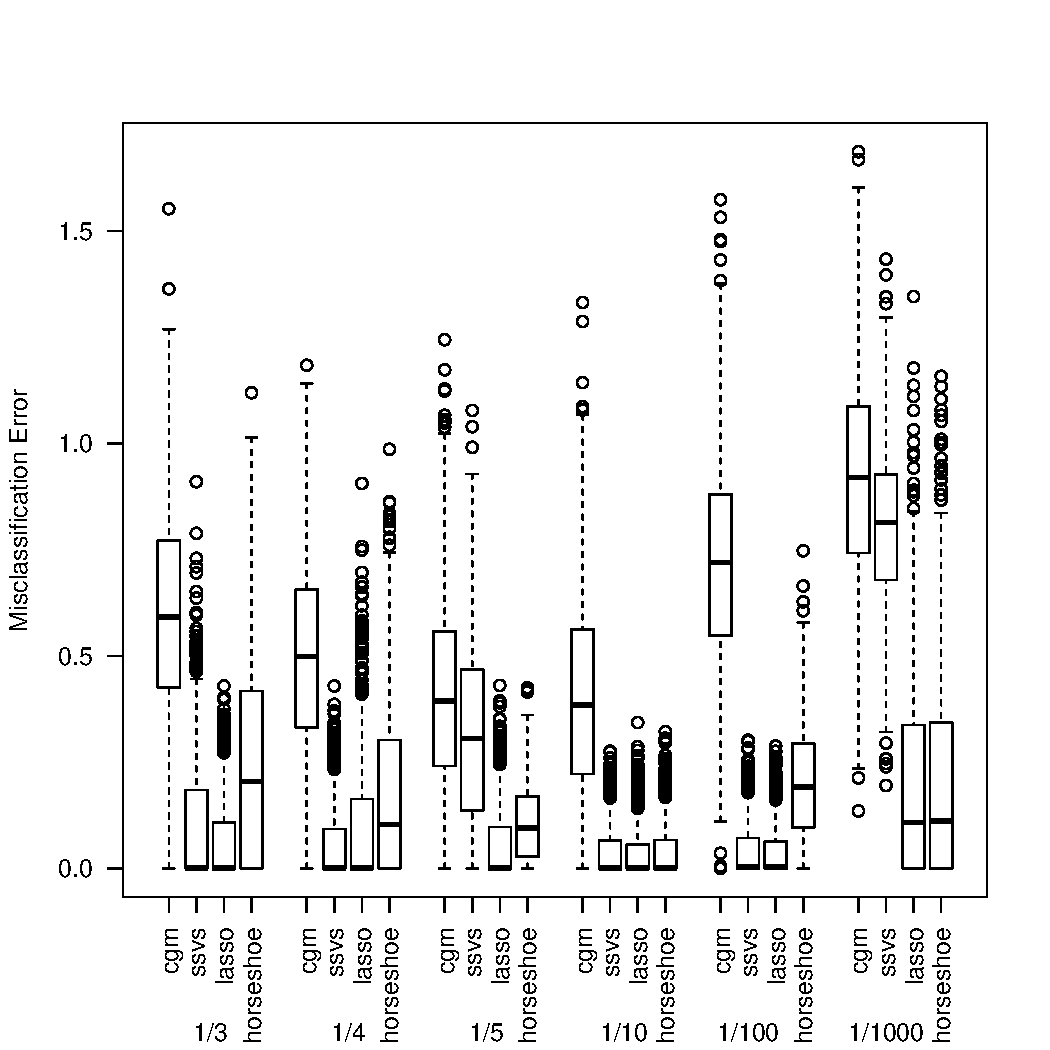
\includegraphics[scale=0.4]{figures/class_imbalance_50_sparsity1.pdf}}
    & \subfigure[]{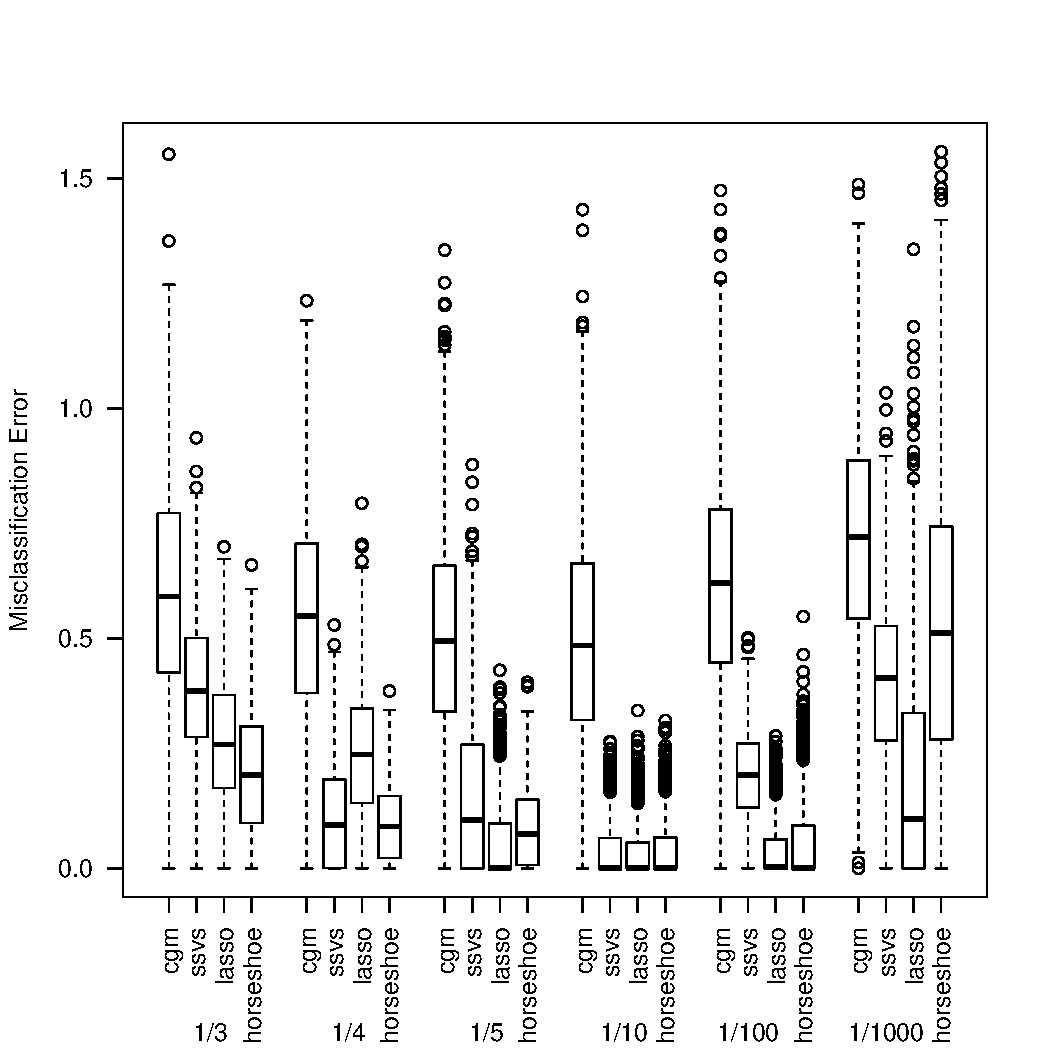
\includegraphics[scale=0.4]{figures/class_imbalance_60_sparsity1.pdf}} \\
  \subfigure[]{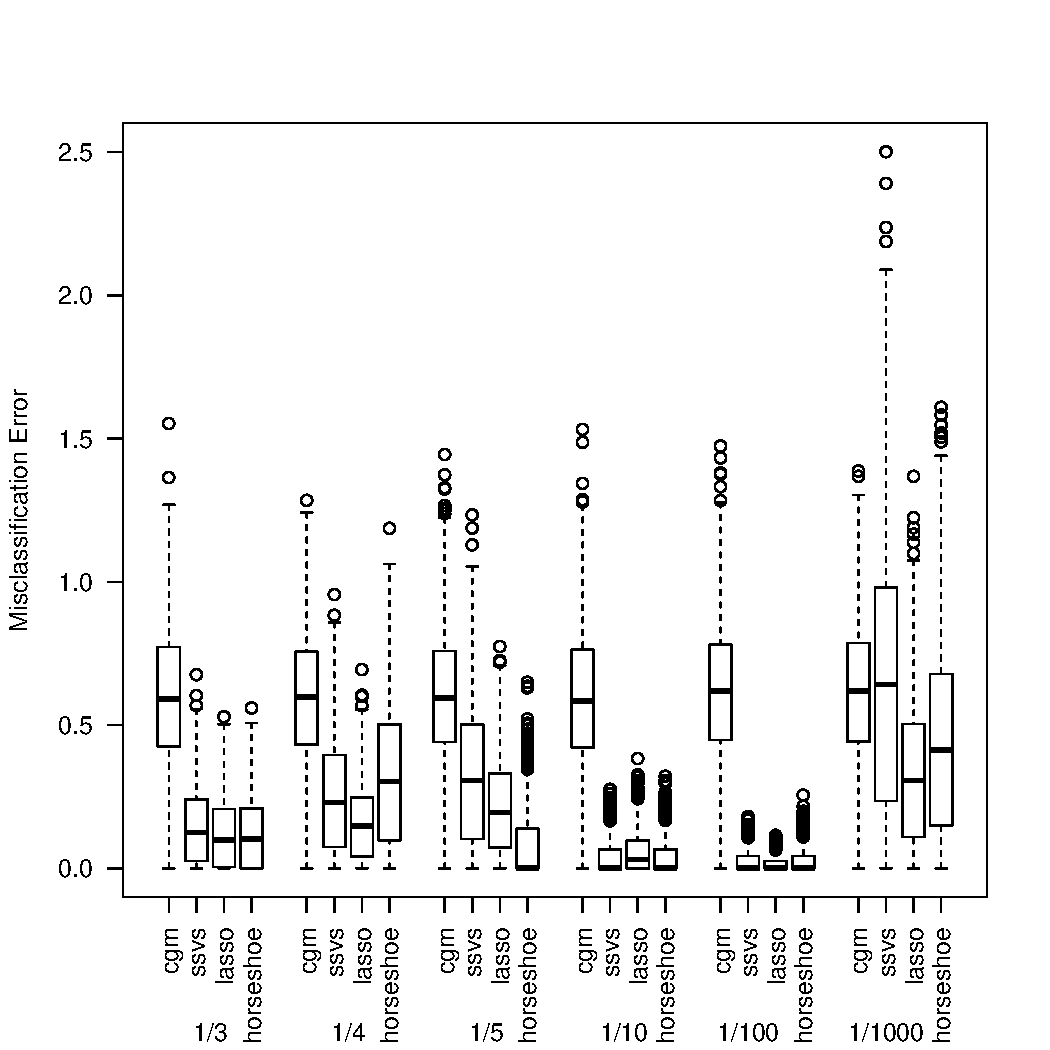
\includegraphics[scale=0.4]{figures/class_imbalance_70_sparsity1.pdf}}
    & \subfigure[]{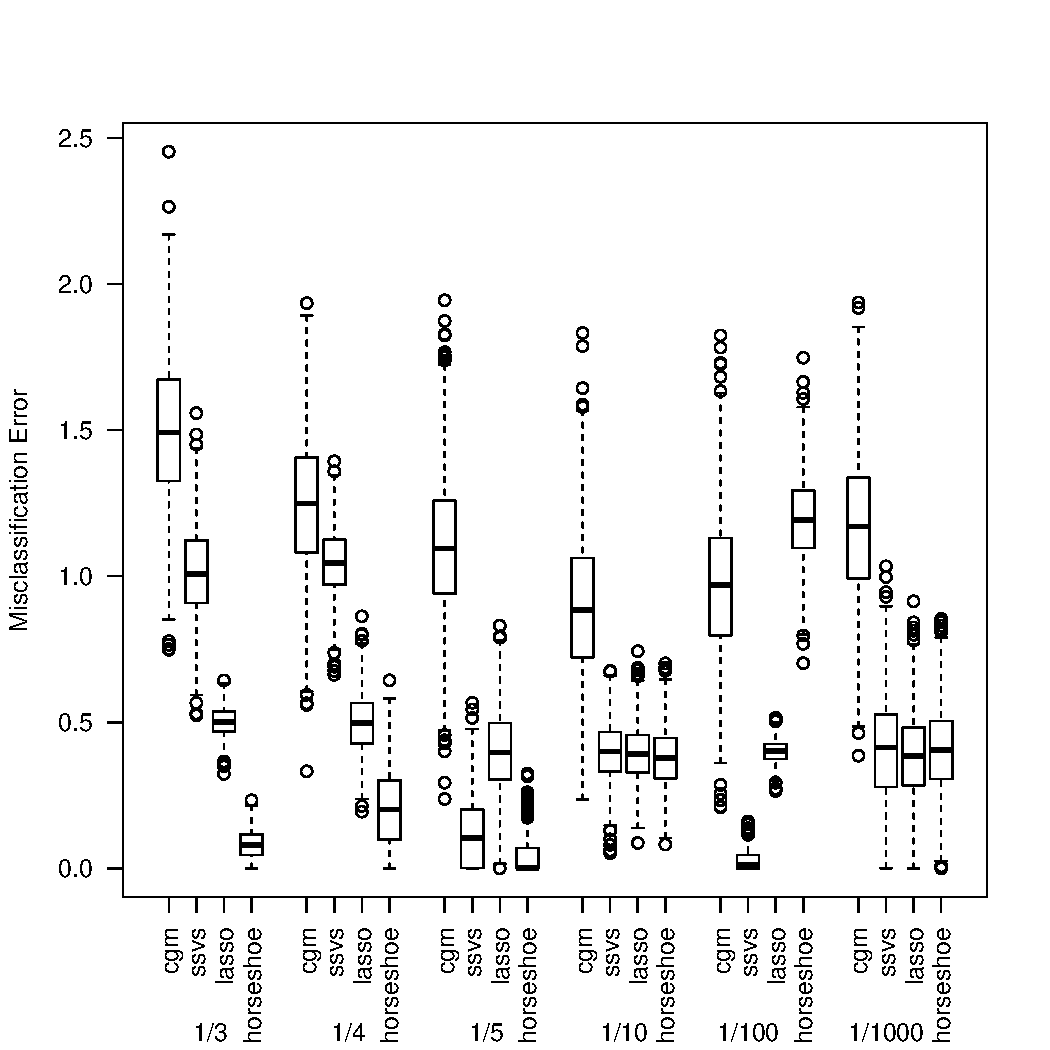
\includegraphics[scale=0.4]{figures/class_imbalance_80_sparsity1.pdf}} \\
   \end{tabular}
\caption{ Box plots of the errors in prediction with the hold out data from the sampled trees after burn-in in the unbalanced simulation study. The three box plots are the prediction errors for the sampled trees for SSVS, lasso, and horseshoe within each set of class probabilities. The fractions displayed with each set of four box plots label the  correspondence with the proportion used to simulate each of the three response classes in the simulated data. Also these proportions are the points on the simplex displayed in Figure \ref{fig:simulated_unbalanced_simplex}. Each letter in the figure, corresponding to the different box plots is a different sparsity value, corresponding to different sparsity levels in the number of covariates. Figure  (a) corresponds to 50\% sparsity, Figure (b) 60\%, Figure (c) 70\%, and Figure (d) 80\%. }
\label{fig:unbalanced_study_results}
\end{center}
\end{figure}

\begin{figure}[H]
\begin{center} 
   \subfigure[]{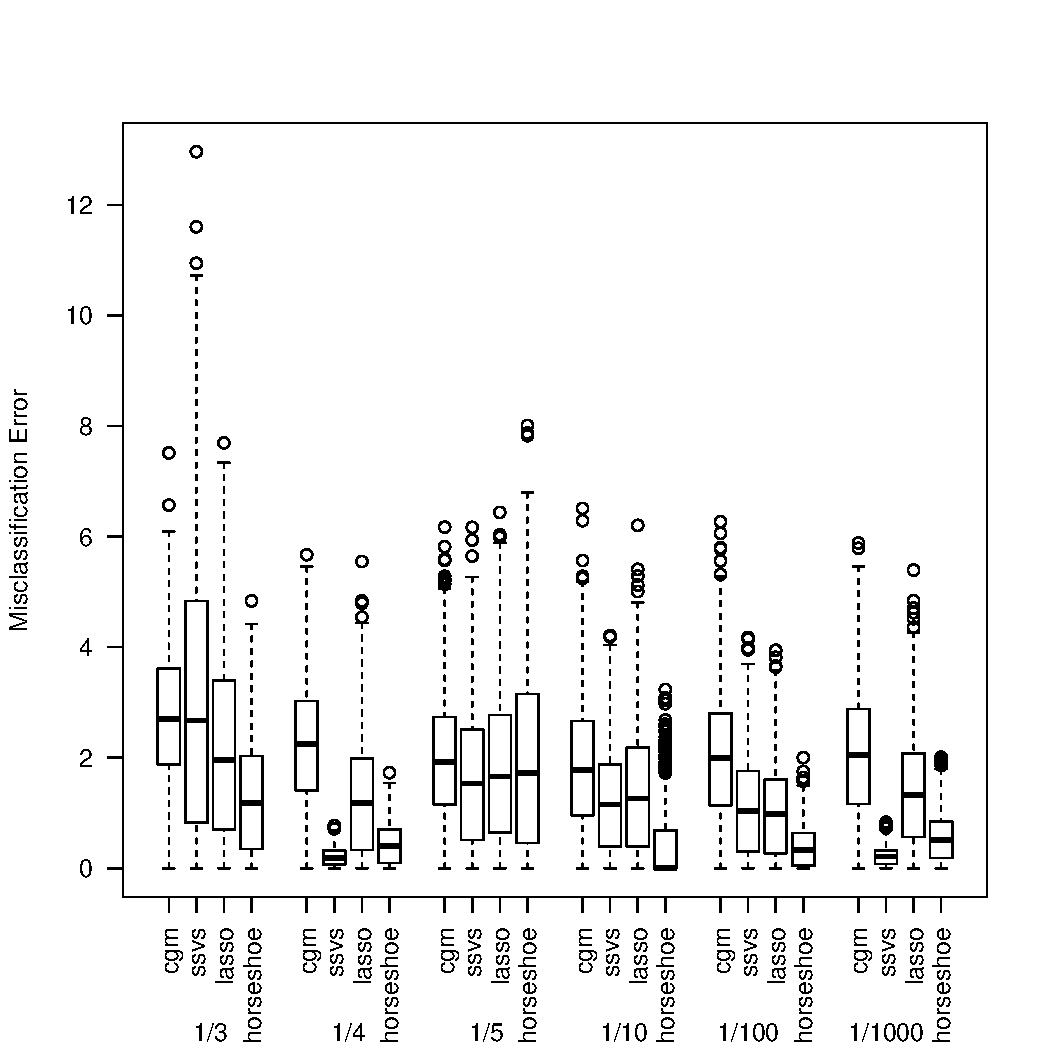
\includegraphics[scale=0.4]{figures/class_imbalance_90_sparsity1.pdf}}
     \subfigure[]{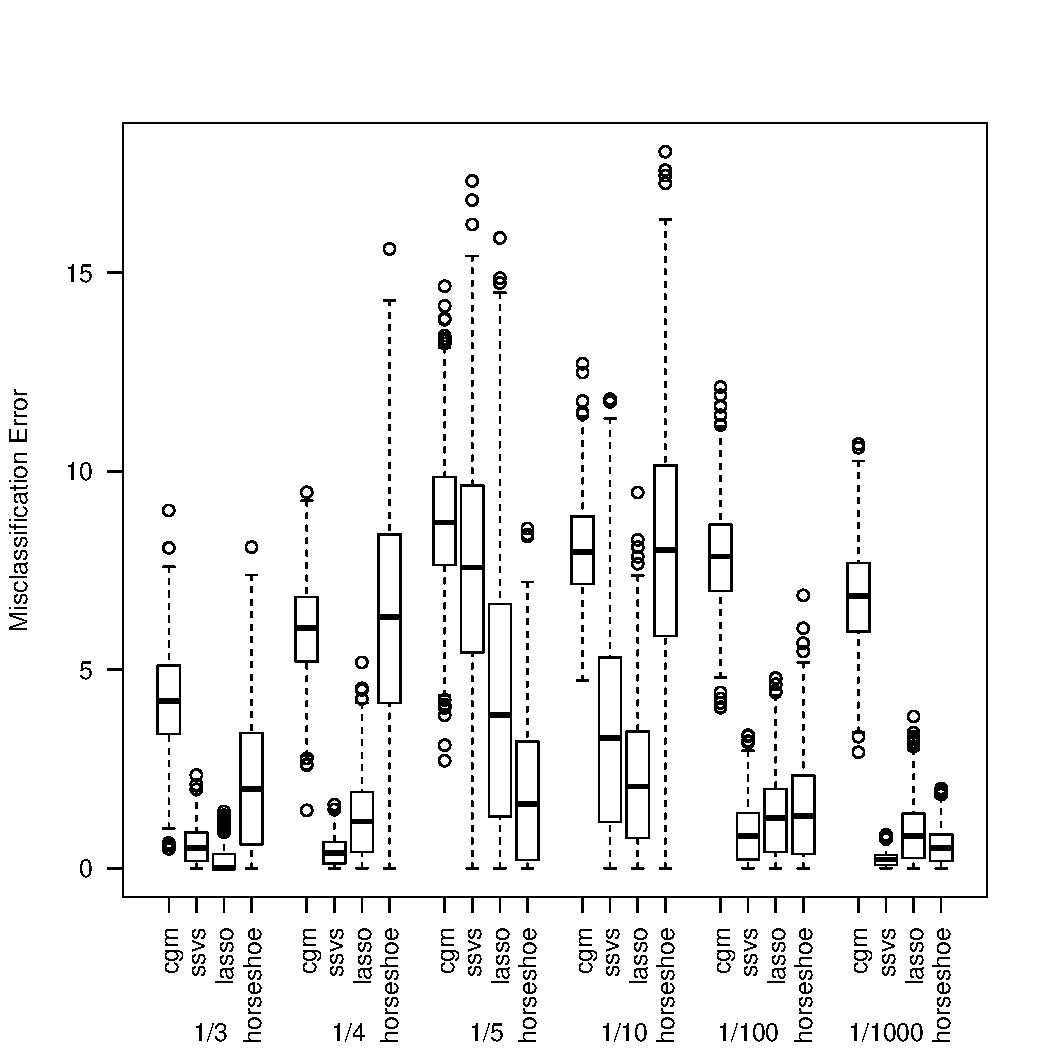
\includegraphics[scale=0.4]{figures/class_imbalance_95_sparsity1.pdf}} \\
\subfigure[]{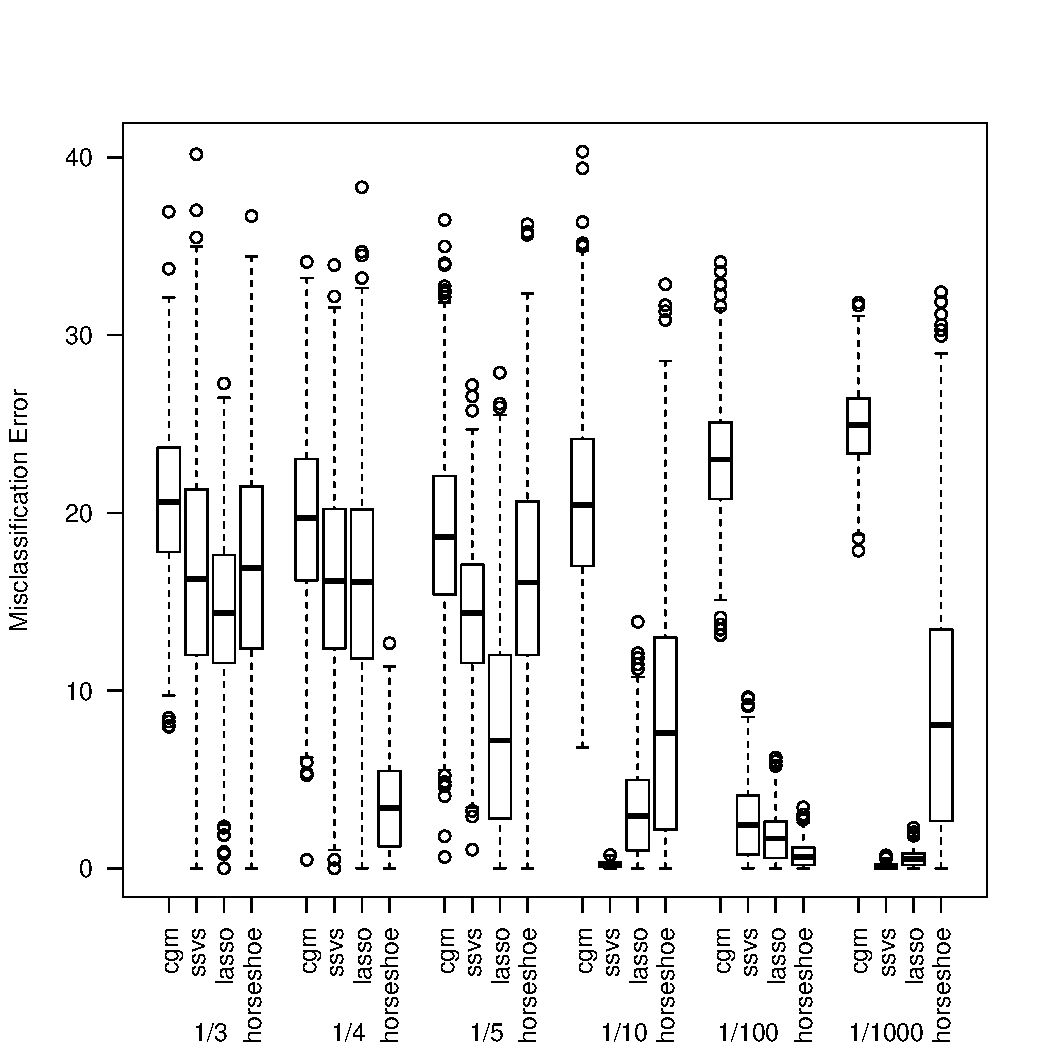
\includegraphics[scale=0.4]{figures/class_imbalance_99_sparsity1.pdf}}
\caption{ Box plots of the errors in prediction with the hold out data from the sampled trees after burn-in in the unbalanced simulation study. This is for the case of 90\% (a) sparsity, 95\% (b) sparsity, and (c) 99\% sparsity. }
\label{fig:unbalanced_study_results2}
\end{center}
\end{figure}

%\begin{table}[H]
%\begin{center}
%\begin{tabular}{cc|c|c|c|c|c|c|}
%\cline{3-8}
%& & \multicolumn{6}{|c|}{Class Imbalance Scenarios }\\  \cline{3-8}
%& & \tiny{(1/3,1/3,1/3)} & \tiny{(1/4,1/4,2/4)} & \tiny{(1/5,1/5,3/5)}  & \tiny{(1/10,1/10,8/10)} &\tiny{(1/100,1/100,98/100)} & \tiny{(1/$10^3$,1/$10^3$,998/$10^3$)}\\\cline{1-8}
%\multicolumn{1}{ |c| }{\multirow{3}{*}{Sparsity 50\%} } & 
%\multicolumn{1}{ |c| }{SSVS} &0.00\%  &0.00\%  & 0.30\% &0.00\%  &0.00\%&0.80\%  \\  \cline{2-8}
%\multicolumn{1}{ |c| }{}&LASSO&0.00\%  &0.00\%  &0.00\%  &0.00\%   &0.00\%  &0.10\%     \\ \cline{2-8}
%\multicolumn{1}{ |c| }{}&HORSESHOE  &0.20\%  &0.10\%  &0.00\%  &0.00\%  &0.20\%  &0.10\%\\ \cline{1-8}
%\multicolumn{1}{ |c| }{\multirow{3}{*}{Sparsity 60\%} } & 
%\multicolumn{1}{ |c| }{SSVS} &0.39\%  &0.10\%  & 0.10\% &0.00\%  &0.20\%&0.40\%  \\  \cline{2-8}
%\multicolumn{1}{ |c| }{}&LASSO&0.27\%  &0.25\%  &0.00\%  &0.00\%   &0.00\%  &0.10\%     \\ \cline{2-8}
%\multicolumn{1}{ |c| }{}&HORSESHOE  &0.20\%  &0.09\%  &0.08\%  &0.00\%  &0.00\%  &0.50\%\\ \cline{1-8}
%\multicolumn{1}{ |c| }{\multirow{3}{*}{Sparsity 70\%} } & 
%\multicolumn{1}{ |c| }{SSVS} &0.13\%  &0.24\%  &0.30\%  &0.04\%  &0.00\%&0.60\%  \\  \cline{2-8}
%\multicolumn{1}{ |c| }{}&LASSO& 0.10\% &0.15\%  &0.20\%  &0.00\%   &0.00\%  &0.30\%     \\ \cline{2-8}
%\multicolumn{1}{ |c| }{}&HORSESHOE  &0.10\%&0.30\%  &0.00\%  &0.00\%  &0.00\%  &0.40\%\\ \cline{1-8}
%\multicolumn{1}{ |c| }{\multirow{3}{*}{Sparsity 80\%} } & 
%\multicolumn{1}{ |c| }{SSVS} &1.012\%  &1.05\%  &0.10\%  &0.40\%  &0.01\%&0.40\%  \\  \cline{2-8}
%\multicolumn{1}{ |c| }{}&LASSO&0.50\%  &0.50\%  &0.40\%  & 0.40\%  & 0.40\% &0.38\%     \\ \cline{2-8}
%\multicolumn{1}{ |c| }{}&HORSESHOE  &0.08\%  &0.20\%  &0.00\%  &0.38\%  &1.20\%  &0.40\%\\ \cline{1-8}
%\multicolumn{1}{ |c| }{\multirow{3}{*}{Sparsity 90\%} } & 
%\multicolumn{1}{ |c| }{SSVS} &2.77\%  &0.20\%  &1.50\%  &1.15\%  &1.01\%&0.20\%  \\  \cline{2-8}
%\multicolumn{1}{ |c| }{}&LASSO&1.97\%  &1.20\%  &1.70\%  &1.40\%   &0.95\%  & 1.30\%    \\ \cline{2-8}
%\multicolumn{1}{ |c| }{}&HORSESHOE  &1.16\%  &0.40\%  &1.84\%  &0.02\%  &0.36\%  &0.50\%\\ \cline{1-8}
%\multicolumn{1}{ |c| }{\multirow{3}{*}{Sparsity 95\%} } & 
%\multicolumn{1}{ |c| }{SSVS} & 0.53\% &0.40\%  &7.51\%  &3.27\%  &0.79\%&0.21\%  \\  \cline{2-8}
%\multicolumn{1}{ |c| }{}&LASSO&0.00\%  &1.20\%  &3.96\%  &2.26\%   & 1.22\% & 0.80\%    \\ \cline{2-8}
%\multicolumn{1}{ |c| }{}&HORSESHOE  &1.96\%  &6.29\%  &1.74\%  &8.08\%  &1.40\%  &0.50\%\\ \cline{1-8}
%\multicolumn{1}{ |c| }{\multirow{3}{*}{Sparsity 99\%} } & 
%\multicolumn{1}{ |c| }{SSVS} &16.52\%  &16.43\%  &14.28\%  &0.20\%  &2.39\%& 0.10\% \\  \cline{2-8}
%\multicolumn{1}{ |c| }{}&LASSO&14.40\%  &16.21\%  &7.36\%  &3.23\%   &1.62  &0.50\%     \\ \cline{2-8}
%\multicolumn{1}{ |c| }{}&HORSESHOE  &16.78\%  &3.36\%  &16.43\%  &7.78\% &0.70\%  &7.78\%\\ \cline{1-8}
%\end{tabular}
%\caption{Class unbalancedness simulation study results, each entry represents the MSE for that scenario and model. The MSE is calculated as $\sum_{i}(\hat{y}_{i}-y_i)^{2}$, where $i$ runs from draw $1,000$ to $10,000$. Thus our burn-in is $1,000$.}
%\label{tab:unbalanced_study_results}
%\end{center}
%\end{table}

Intuitively, the results of Figures \ref{fig:unbalanced_study_results} and \ref{fig:unbalanced_study_results2} make sense. The less sparse the true model, the easier the model can classify the categories. Sparse models are not terribly difficult to classify. However, cases of extreme sparsity, such as those where 99+\% sparsity exists, are likely to have a far greater error rate. Interestingly, the degree of imbalance in the true, underlying model appear to affect the error as well. The explanation here is that, a decision tree can more easily partition a subset of the covariate space to classify responses that are rare as compared to more prevalent responses.

The results here are somewhat inconclusive on which specific model, ssvs, lasso, or horseshoe is best in a given scenario. It appears from the unbalanced simulation studies that, aside from Monte Carlo variability, there is no clear winner amongst the three ALoVaS models. It does appear that given a certain sparsity and perhaps other characteristics of the underlying model, such as correlation or class unbalanceness, it may be better to choose one type of ALoVaS model over the others. However, this information seems unlikely to be known \emph{a priori} except in special circumstances. Moreover, any of the ALoVaS methods is likely to prove useful and provide improvements over the traditional Bayesian decision tree algorithm proposed by CGM. 

\section{Case Study}\label{sec:real_data}

In this section we compare the ALoVaS method against the CGM approach, a variable importance (VIMP) based frequentist method \cite{ishwaran2010high}, and a non-decision tree based approach, the logistic-lasso. We compare these methods using the publicly available internet ads dataset from the UCI data repository \cite{Frank:2010uq}. The internet ads data set contains 1558 covariates, some numeric and some categorical. The data set was first used in a paper by Kushmerick \cite{kushmerick1999learning} and has since been used in several statistical classification studies. A more complete description of the data and references to other papers using this dataset can be found at the UCI machine learning repository website, at the following link: \url{https://archive.ics.uci.edu/ml/datasets/Internet+Advertisements}.

As noted by Kushmerick \cite{kushmerick1999learning}, there are several reasons for wanting to remove advertisements from webpages. Some reasons are: images tend to dominate a pages total download time, users dislike paying for services indirectly through advertisers preferring direct payment for services rendered, and malicious software can be unintentionally placed on a user's machine through images masked as advertisements. 

		\begin{table}[H]
\begin{center}
\begin{tabular}{|c|c|} \hline
Model & Error \\ \hline
ALoVaS-SSVS&$7.48 \pm 2.01$\%\\ \hline
ALoVaS-Lasso &$5.12 \pm 1.38$\% \\ \hline
ALoVaS-Horseshoe& $5.40 \pm 3.22$\% \\ \hline
VIMP& $15.30 \pm 4.10$\%\\ \hline
CGM& $7.20 \pm 3.57$\%\\ \hline
Logistic-lasso&$11.20 \pm 4.11$\%\\ \hline
\end{tabular}
\caption{Class unbalancedness simulation study results, each entry represents the MSE for that scenario and model. }
\label{tab:ads_misclass}
\end{center}
\end{table}

	
\begin{figure}[H]
\begin{center} 
\begin{tabular}{cc}
 \subfigure[]{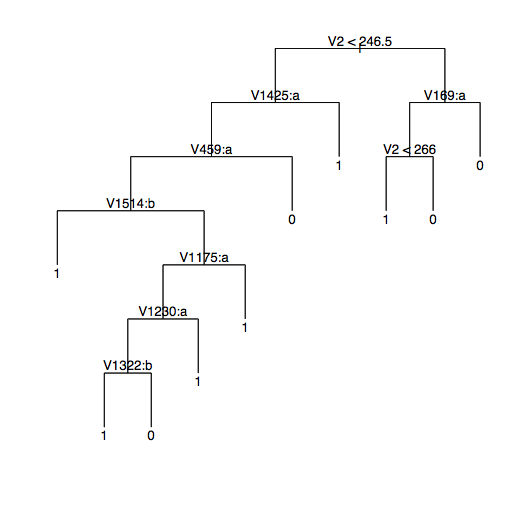
\includegraphics[scale=0.35]{figures/CGM.png}}
    & \subfigure[]{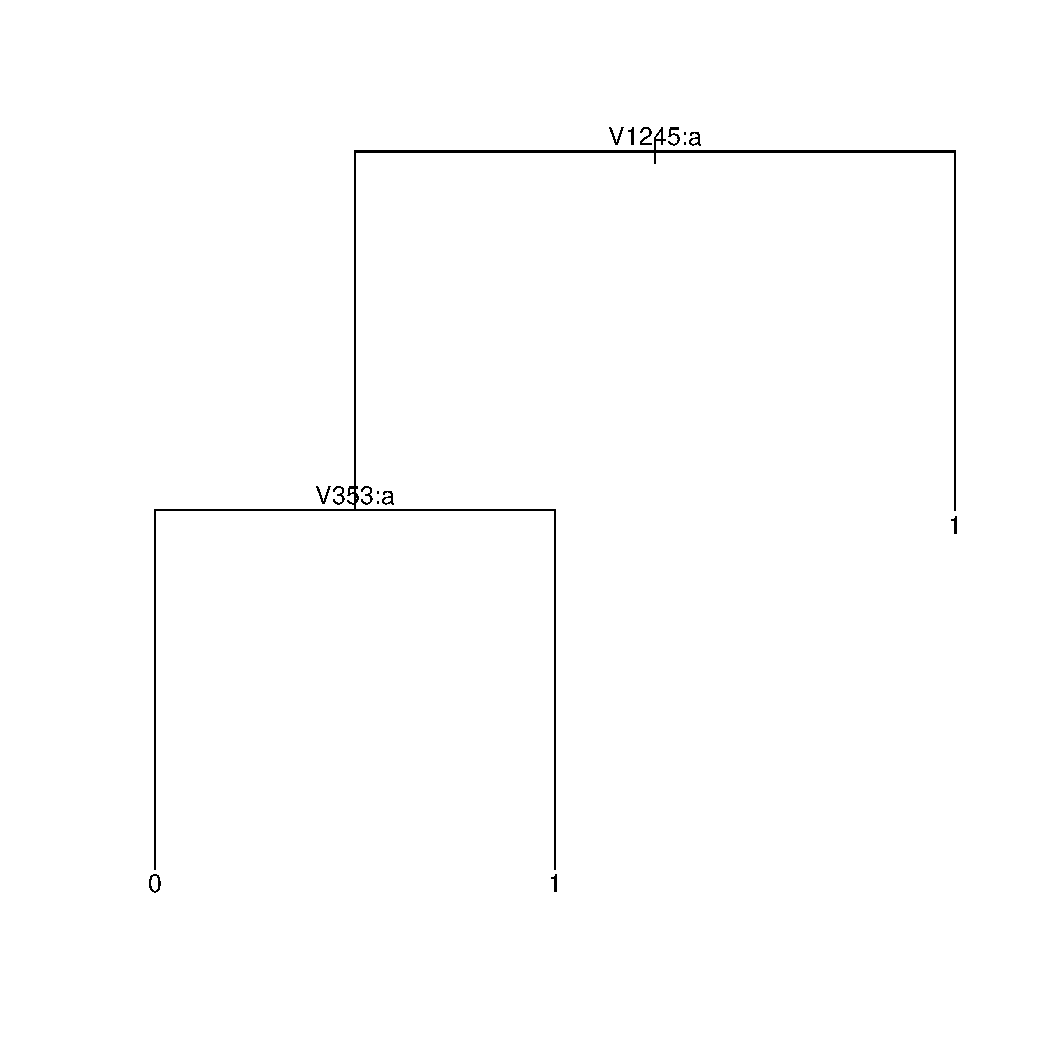
\includegraphics[scale=0.35]{figures/ads_dataset_lasso_tree.pdf}} \\
  \subfigure[]{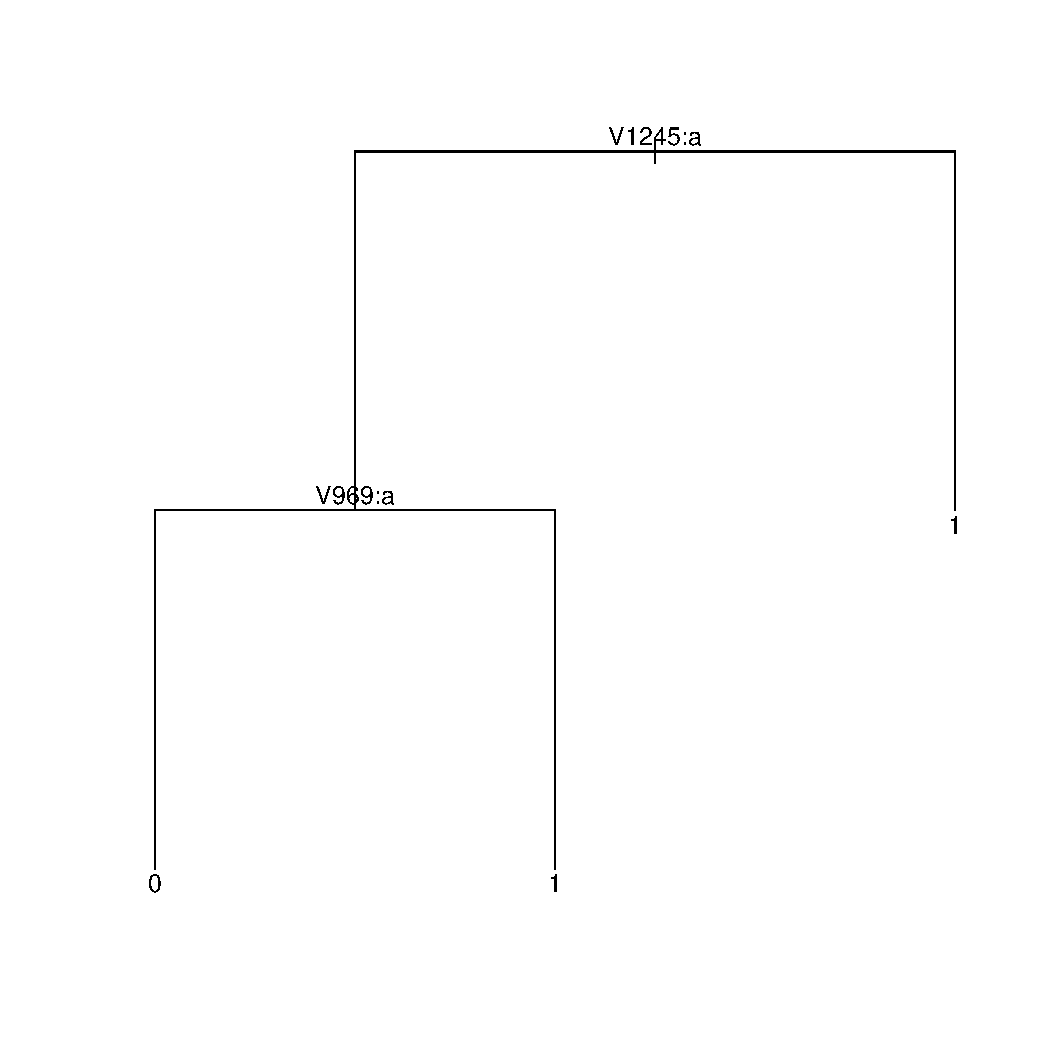
\includegraphics[scale=0.35]{figures/ads_dataset_ssvs_tree.pdf}}
    & \subfigure[]{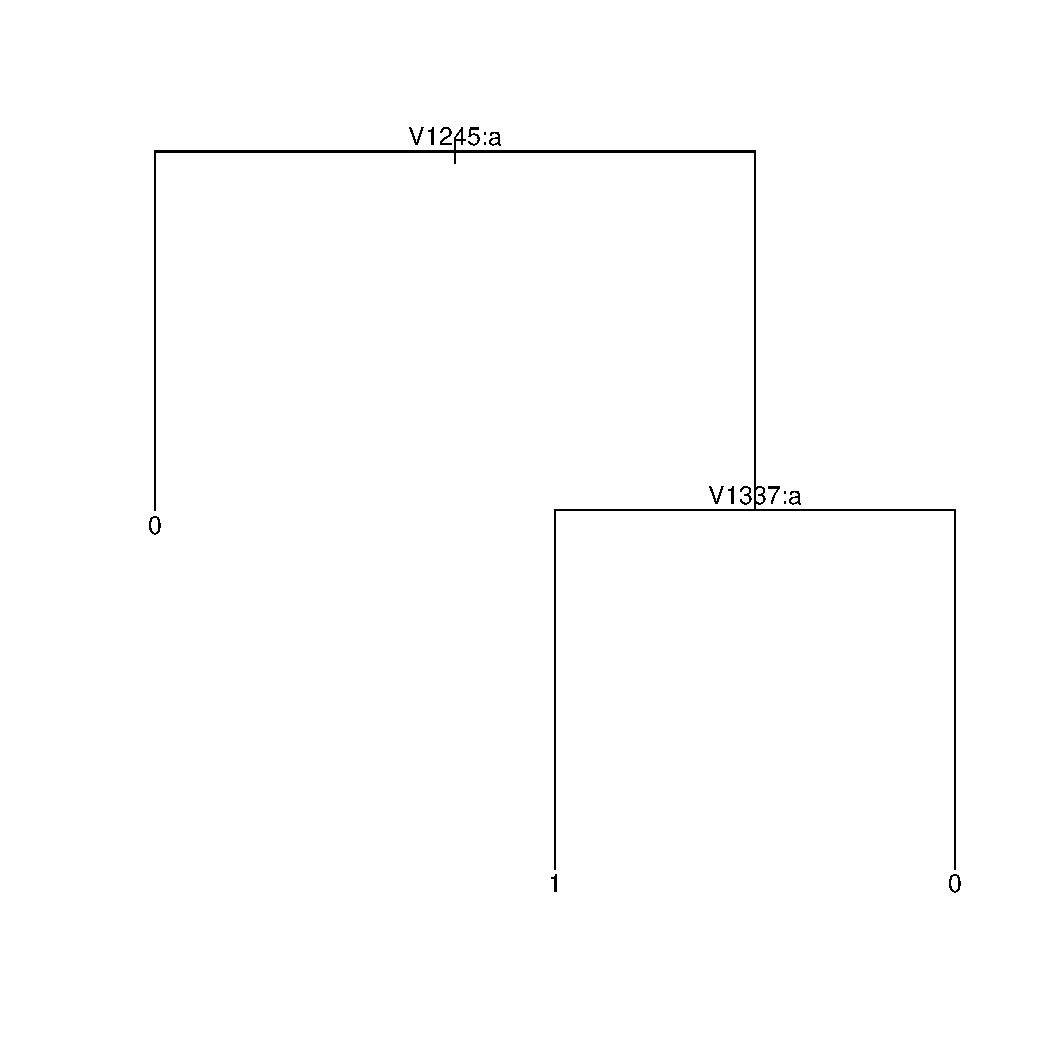
\includegraphics[scale=0.35]{figures/ads_dataset_horseshoe_tree.pdf}} \\
    \end{tabular}
\caption{The  decision trees fitted to the internet ads dataset. The CGM (a) is much deeper than the remaining three trees fit using the ALoVaS method. The SSVS (b), Lasso (c) and horseshoe (d) all select the 1245th variable along with a second variable. The second variable differs in each of the three ALoVaS variants we use but the fact that the 1245th variable is common to all three gives further credence to the claim that a choice between the SSVS, lasso, or horseshoe types of ALoVaS is largely a choice of personal preference. }
\label{fig:unbalanced_study_results_trees}
\end{center}
\end{figure}
	
	
%	\begin{figure}[H]
%  \centering
%  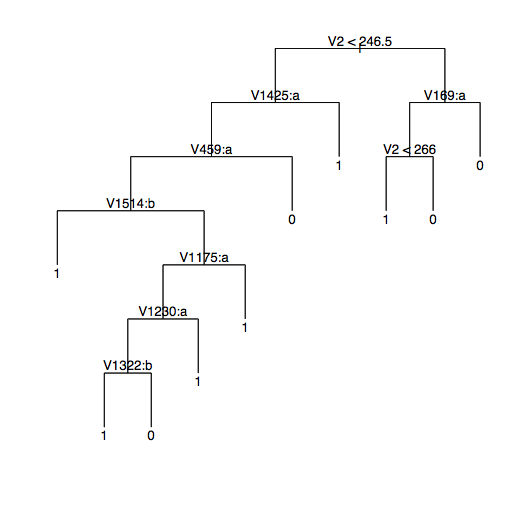
\includegraphics[width=4in]{figures/CGM.png}
%  \caption{The tree fit using the CGM approach.}
%  \label{fig:CGM_tree}
%\end{figure}	
%
%%	\begin{figure}[H]
%%  \centering
%%  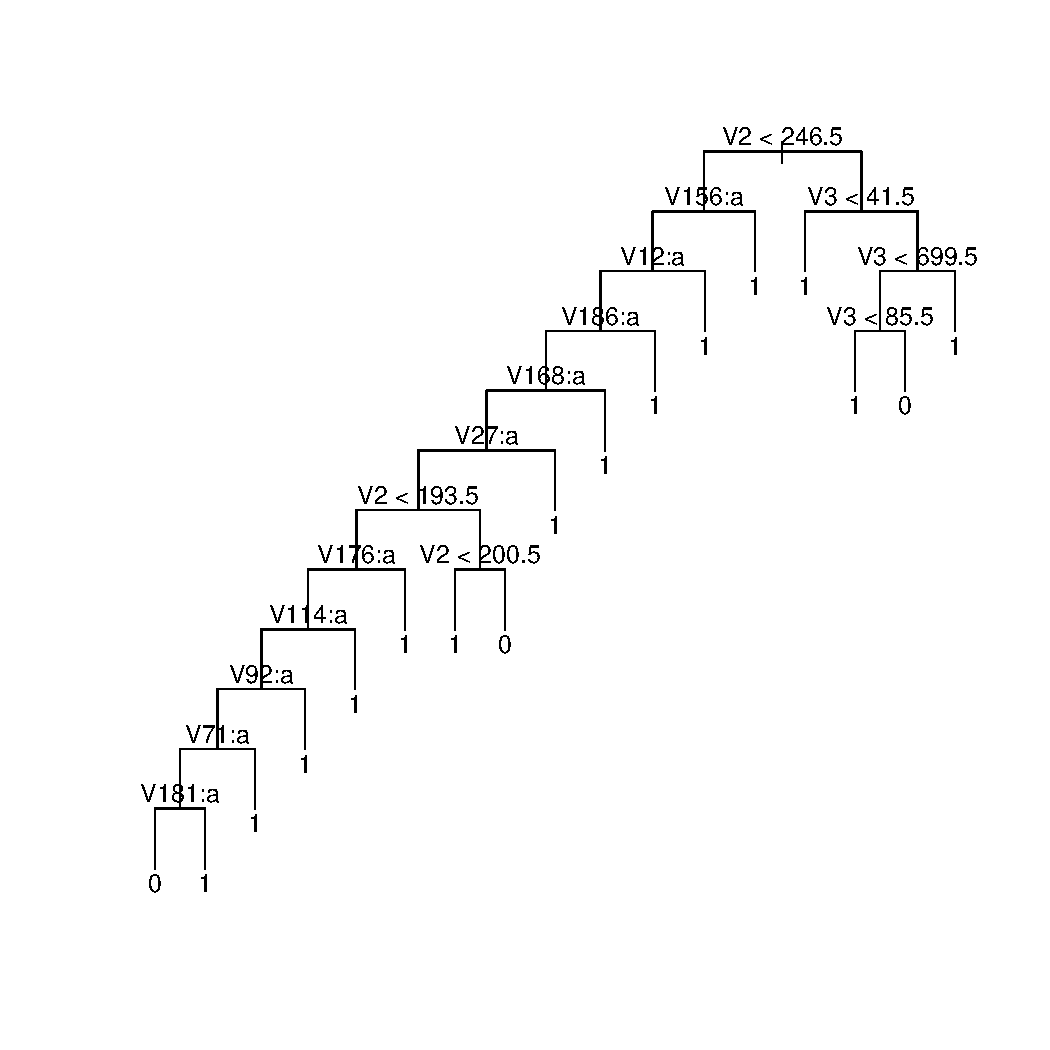
\includegraphics[width=4in]{figures/ad_tree.pdf}
%%  \caption{The tree fit using the greedy approach.}
%%  \label{fig:greedy_tree}
%%\end{figure}	
%
%	\begin{figure}[H]
%\begin{center}
%  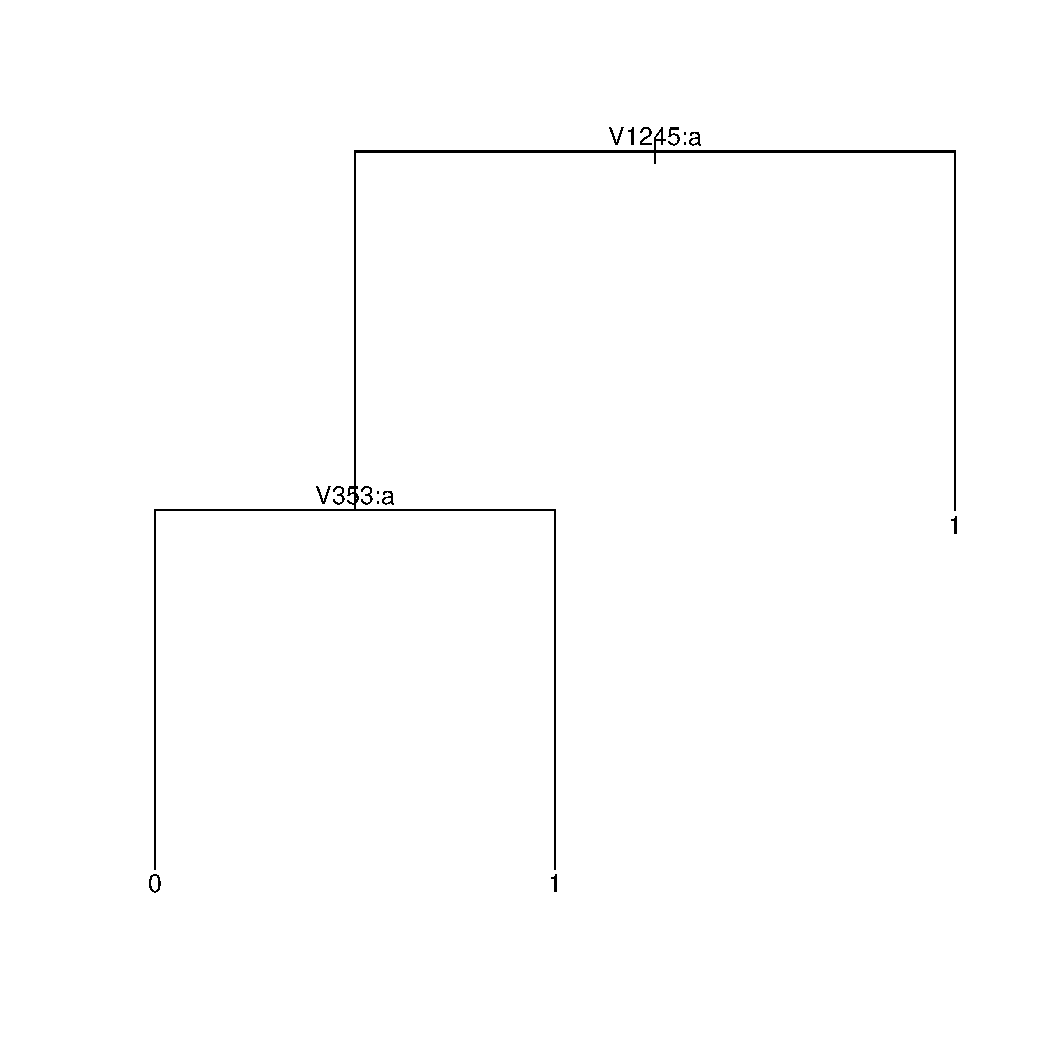
\includegraphics[scale=0.3]{figures/ads_dataset_lasso_tree.pdf}
%  \caption{The lasso ALoVaS decision tree. }
%  \label{fig:horseshoe_ads_tree}
%  \end{center}
% \end{figure}		
%
%	\begin{figure}[H]
%\begin{center}
%  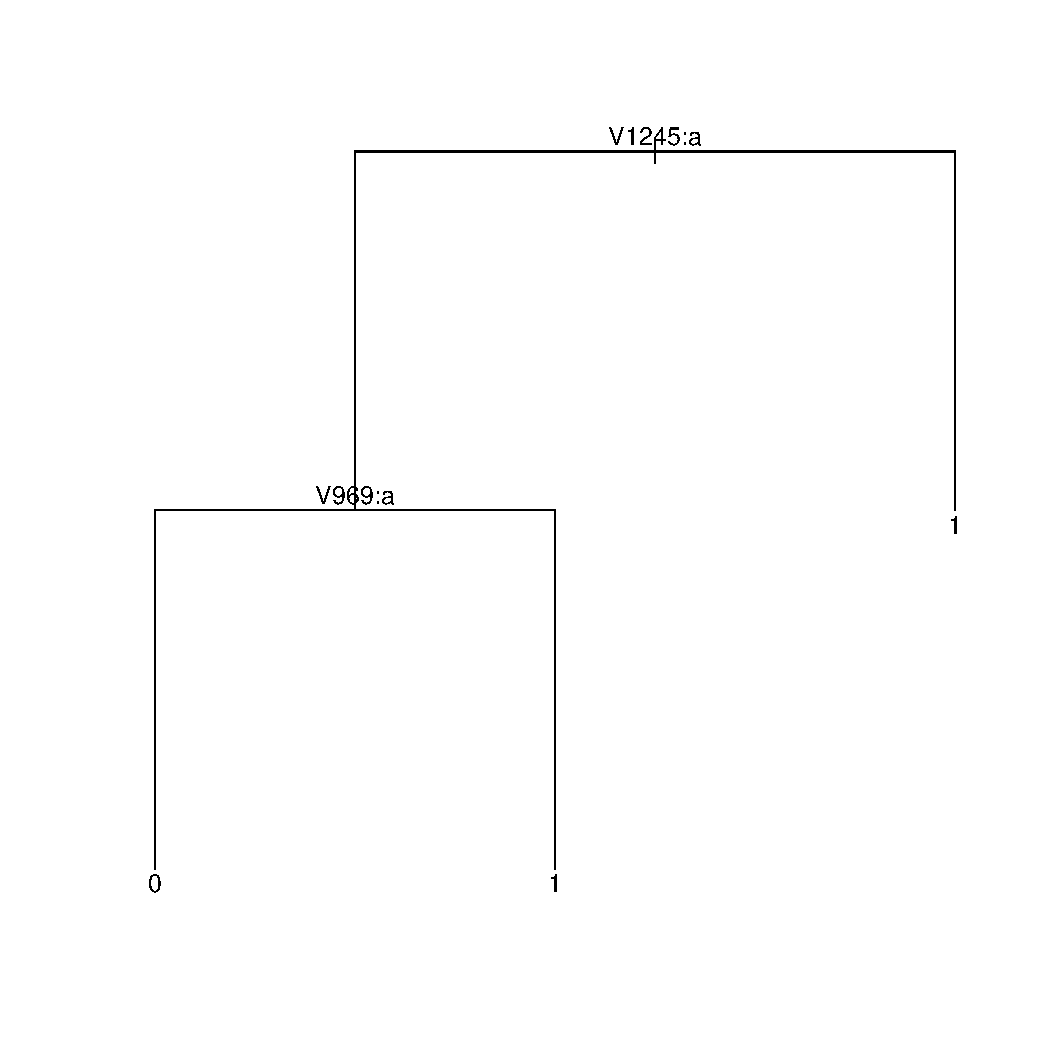
\includegraphics[scale=0.3]{figures/ads_dataset_ssvs_tree.pdf}
%  \caption{The ssvs ALoVaS decision tree. }
%  \label{fig:ssvs_ads_tree}
%  \end{center}
% \end{figure}	
%
%	\begin{figure}[H]
%\begin{center}
%  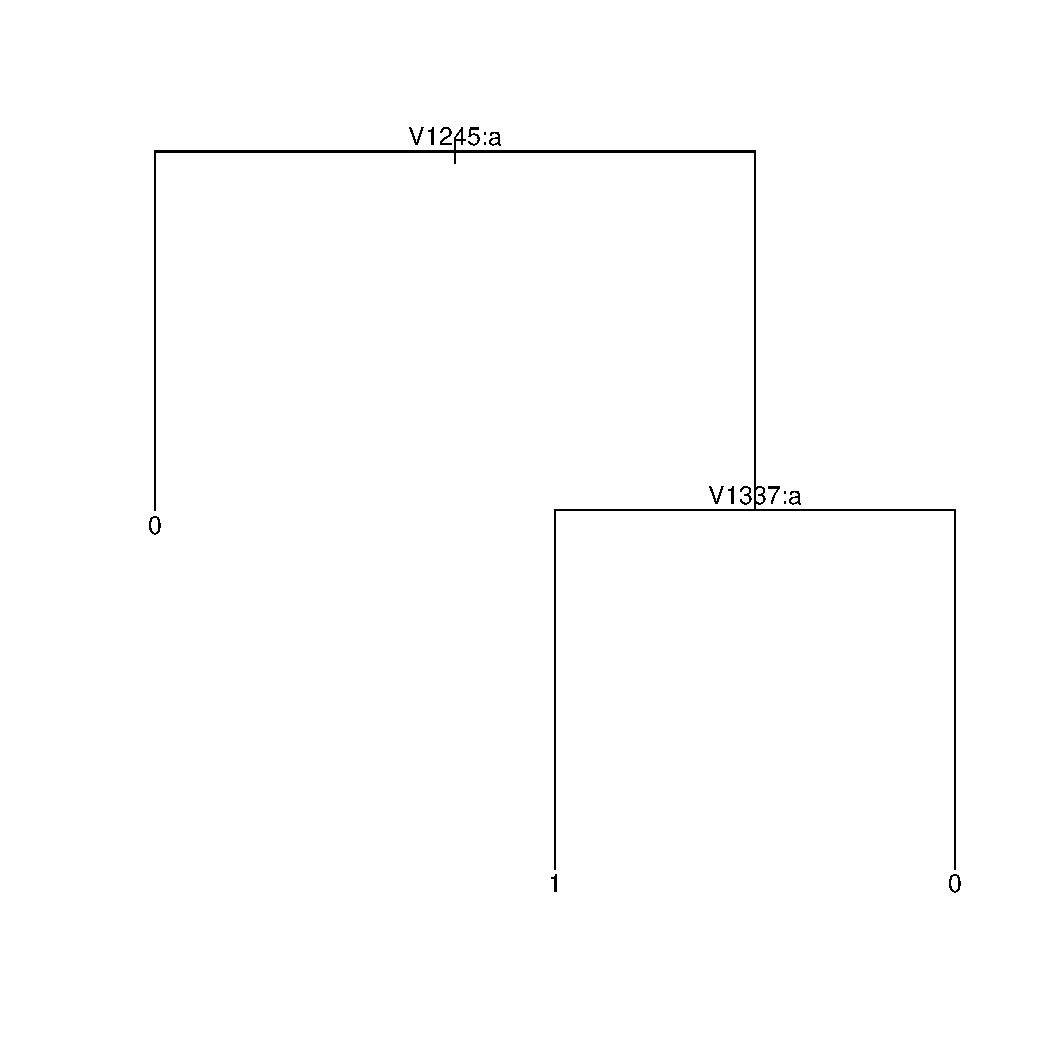
\includegraphics[scale=0.3]{figures/ads_dataset_horseshoe_tree.pdf}
%  \caption{The horseshoe ALoVaS decision tree. }
%  \label{fig:horseshoe_ads_tree}
%  \end{center}
% \end{figure}		
%		
		We use a random subset of the internet ads data to fit a CGM tree and an ALoVaS tree. We first remove all observations that contain missing values. We then take a 50\% random sample of training and test data. The MSE is calculated as $\sum_{i}(\hat{y}_{i}-y_i)^{2}$/10,000, where $i$ runs from draw $1,000$ to $11,000$. Thus our burn-in is $1,000$. Figure \ref{fig:unbalanced_study_results_trees} shows the estimated trees. The misclassification probabilities are calculated by dropping all data points from the test data set through the trees built using the training data. The resulting trees are fit using only the training data.  In this example we do not know the ground truth, so comparison of misclassification rates against a ground truth is not possible. Nevertheless, we compare misclassification rates amongst the models shown in Table \ref{tab:ads_misclass}. 
		
		From the misclassification errors shown in Table \ref{tab:ads_misclass}, it is clear that some of the trees compete with each other in terms of prediction. However, once we examine the images of the fitted decision trees in Figure \ref{fig:unbalanced_study_results_trees} ,we see that there is a dramatic difference in terms of the complexity of the tree for a given prediction error. The ALoVaS models are able to select trees with maximum depth of 2 and achieve comparable error rates to the CGM tree which has more splits on more variables. 
		
		Comparing the different decision trees selected by the three types of ALoVaS methods indicates that there is little practical difference between the SSVS, lasso, and horseshoe ALoVaS methods. Additionally, the variables selected by the three ALoVaS methods are very similar. Hence, the ALoVaS method is relatively insensitive to the regularization method used. Saying that, it is clear that there is a substantive performance increase over non-sparse competitors such as the CGM method and the logistic lasso. CGM is a nonlinear dense method, whereas logistic lasso is a linear, sparse method. In a nutshell, ALoVaS merges the benefits of both CGM and the lasso. The variable 1245 indicates that the webpage includes in the url the term `psu.edu', showing that at the time the internet ads dataset was collected, Penn state's website was hosting advertisements. The other variable that is commonly occurring is variable 353, which indicates that the url term contains the text string `images+ads', which seems to be an obvious choice of predictor. Further the variable 1337 indicates that the url string contained the set of characters `sj', which is a difficult set of characters to interpret and is likely ancillary information. 
		
		The take home point of this section is that, not only is the ALoVaS method a useful conceptual method for performing variable selection when fitting Bayesian decision trees, but it is also practically useful. The ALoVaS method is capable of handling data with a large number of covariates and of performing covariate filtering by choosing various covariates. As a byproduct of the fitting method we also generate a sampled set of covariate selection probabilities which can be used if the method is to be compared with other methods that perform variable selection and use a similar approach. 

\section{Conclusions}\label{sec:Conclusion}

A lot of press is given to variable selection methods, both in terms of theoretical properties and in terms of practical results. However, these applications nearly always implement linear or generalized linear models. Non-linear models, such as decisions trees, are mathematically less tractable and thus theoretical results are more difficult to derive. Our ALoVaS method facilitates variable selection methods familiar to the researcher and allows their use with decision tree models. In non-sparse settings our method experiences similar difficulties as those experienced by methods such as the lasso and horseshoe. This is not a limitation of our method \emph{per se} but rather an effect of model misspecification. 

One difficulty with the ALoVaS method proposed in this article is that exact zeros and ones are impossible unless $\Pr(\mu_j \in \{-\infty,\infty\})\neq 0$. This is a difficulty of all models using the ALN density and was noted by Atchison and Shen \cite{atchison1980logistic}, as a point in need of remedy. Although exact zero covariate selection probabilities are not theoretically possible with our model, we are able to create sparse, simple decision trees via the ALN density by estimating zero probabilities as numerically negligible. 

Of course, there are other distributions defined on the simplex that one might find useful to use for variable selection with decision trees. Perhaps using one of the distributions on the simplex from J\o rgensen's \cite{jorgensen1997theory} dispersion model apparatus would be a fruitful line of research. However, analytical intractability would result from using this type of distribution. Additionally, one would need to generalize the definition of this density to a simplex on more than 2 dimensions. Perhaps, if other densities on the simplex are deemed applicable, the application of those densities to decision tree variable selection could follow a line of reasoning similar to that described here. 

%future work? 
There remain several avenues of future work based on the findings documented in this manuscript. We list three:

\begin{itemize}
\item Explore other regularization methods that have non-zero probability of setting $\mu_j=0$. 
\item Study the effect of imposing normality on the split counts, $s_{ij}$ instead of a Poisson or negative binomial model. 
\item Study the effects of multiplicity adjustments, false positives, and false negatives in the models detailed. 
\end{itemize}

Regarding the first comment, the model proposed by Bhattacharya, Pati, Pillai, and Dunson \cite{bhattacharya2012bayesian} might be a useful first step. For the second item listed, the Gibbs sampling method proposed by Polson, Scott, and Windle \cite{polson2013bayesian} seems to be the way forward. Finally, regarding the last item, the arguments in Scott and Berger \cite{scott2010bayes}, as well as Efron's many articles and book length treatise \cite{efron2009empirical,efron2004large,efron2007correlation,efron2010large}, are logical starting points. 

In this Chapter and the previous Chapter we proposed a novel framework for linking variable selection or regularization methods from linear models with variable selection in decision tree models. Moreover, we compared simulated and real data using our proposed ALoVaS method against common competitors, such as the logistic lasso and the CGM decision tree approach. Our ALoVas method showed improved prediction errors over the logistic lasso and the CGM methods. Moreover, our method provided sparser, less deep decision trees compared to other decision tree methods. This allows easier interpretation of the model both for trained analysts and for non-technical stakeholders. While it is inevitable that limitations exist with all methods, it appears that for sparse data generating processes where a simple structural model is desired, our ALoVaS method is to be preferred.  
